\chapter{Public-Key Cryptography}\label{ch:pub_key_crypto}

%------------------------------------------
\section{Introduction}\label{sec:pubkey:intro}
%------------------------------------------

Public-key methods use the following functions for encrypting and decrypting:

\begin{align*}
    KGen(1^n)  & \rightarrow (sk, pk) \\
    Enc(pk, m) & \rightarrow c        \\
    Dec(sk, c) & \rightarrow m        \\
\end{align*}

Often, the public key can be computed efficiently from the secret key $f(pk) \rightarrow sk$.
But for security, it is required that the reverse of this function $f^{-1}$, which computes the secret key from the public key is \emph{not} efficiently computable.
We call such a function, that can only be efficiently computed in one direction a \emph{one-way function} (OWF).

%----------------------------------------
\section{One-Way Functions}\label{sec:owf}
%----------------------------------------

A one-way function (OWF) is a function $f: \{0,1\}^* \rightarrow \{0,1\}*$ that can be efficiently computed but its inverse function cannot be efficiently computed.

Formally speaking, a function $f$ is one-way if it has the following two properties:

\begin{enumerate}
    \item There is an efficient algorithm PPT for computing values $f(x)$ for all allowed input parameters $x$.
    \item For all efficient PPT algorithms A their success probability in the below security game $G^{inv}_{f,A}$ is negligible.
\end{enumerate}

$G^{inv}_{f,A}$ is defined as follows:

\begin{align*}
    \{0,1\}^\lambda & \$\rightarrow x \\
    f (x)           & \rightarrow y   \\
    A(1^\lambda, y) & \rightarrow x'  \\
    return f(x) == x'
\end{align*}

\textbf{Note 1:} This game does not require the adversary $A$ to find the value $x$ used but merely requires it to find a value that produces the output for $f$ i.e. a collision.

\textbf{Note 2:} This assumes that there are problems that are hard to compute (NP-hard). This is an assumption that holds so far but is not proven.

%---------------------------------------------
\section{Number Theory}\label{sec:number_theory}
%---------------------------------------------

\subsection{The Modulo Operator}

The modulo operator allows us to calculate with residual rings, which means that all values will never exceed the number $m-1$ for a residual ring $Z_m$.
We define addition and multiplication, such that they produce a value $x \in Z_m$ such that:

\begin{align*}
    a + b & = c mod m \quad |\quad \exists i \in Z: \quad a + b = c + i \cdot m     \\
    a + b & = c mod m \quad |\quad \exists i \in Z: \quad a \cdot b = c + i \cdot m
\end{align*}

\subsection{Groups}

A group is a combination $(G,\circ)$ of a set $G$ and an operation $\circ$ with the following 4 characteristics:

\begin{itemize}
    \item Closure: $a \circ b \in G \quad | \quad \forall a,b \in G$
    \item Associativity: $a \circ (b \circ c) = (a \circ b) \circ c \quad \forall a,b,c \in G$
    \item There exists an identity element (neutral element) $n$ such that $a \circ n = n \circ a = a \quad \forall a \in G$
    \item There exists an inverse element $a^{-1}$ for all elements $a$ in $G$ that can turn $a$ into the neutral element if combined with the operation $\circ$: $\exists a^{-1} \in G: \quad a \circ a^{-1} = a^{-1} \circ a = n \quad \forall a \in G$.
\end{itemize}

We call a group an abelian group if it is a group for which the operation $\circ$ over $G$ is commutative for all elements in $G$:
$a \circ b = b \circ a \quad \forall a,b \in G$.

Groups, or abelian groups, are nice to work with in cryptography.
Unfortunately, residual rings $Z_m$ are generally not groups if paired with the multiplication operator $(Z_m,\cdot)$ because they do not have inverse elements for all elements in $Z_m$. For example, each group $Z_m$ contains the value $0$, but no number can be multiplied by $0$ to produce the neutral element, which is $1$.
Additionally, depending on $m$, other elements might have no inverse element as well.

For this reason, we would like to reduce the set $Z$ to a set $Z_m^*$ that only contains all invertible elements of $Z_m$, thus making it a group.
The invertible elements of $Z_m$ are exactly all elements for which the greatest common divisor ($gcd$) is equal to $0$.
For instance, for the residual ring $Z_6 = \{0, 1, 2, 3, 4, 5\}$, the reduced group would be $Z_6^* = \{1, 5 \}$.

The number of elements in $Z_m^*$ is well defined for a couple of cases for prime numbers $p,q$ and positive integers $k$:

\begin{itemize}
    \item $|Z_p^*| = p-1$ (all elements of $Z_m$ except $0$)
    \item $|Z_{p^k}^*| = p^k - \frac{p^k}{p}$ (all elements except all multiples of p in $Z_{p^k}$)
    \item $|Z_{p \cdot q}^*| = |Z_{p}^*| \cdot |Z_{q}^*|$\footnote{This can be proven as follows: $\Phi(p \cdot q) = p \cdot q - (p-1) - (q-1) - 1 = p \cdot q - (p-1) - q  + 1 - 1 = (p-1)q - (p-1) = (p-1) \cdot (q-1) = \Phi(p) \cdot \Phi(q)$. These are all elements contained in $Z_{p,q}$ except all multiples of $p$ (there are $q-1$ of those and $q$ (there are $p-1$ of those). And also the element $0$ has to be subtracted.}
\end{itemize}

\textit{Def:} The \emph{order} of a group $(G, \circ)$ is the number of the elements in $G$: $ord(G) = |G|$.

\textit{Def:} The \emph{order} of an element $a \in G$ of a group $(G, \circ)$ is the number of elements that can be generated by applying the operation $\circ$ to $a$ and $a$ in $G$.

\textit{Def:} A group $(G, \circ)$ is \emph{cyclic} there exists an element $g \in G$, which we call the generator of the group, that can generate all elements of the group. This means that $ord(g) = ord(G)$.
It can be proven all groups $(Z_p^*, \cdot)$ with prime numbers $p$ are cyclic.

In cryptography, we would like to have a group $(G, \cdot)$ that is cyclic \emph{and} has a prime number of elements.
If we choose $Z_p^*$ with a prime $p$, we have a cyclic group. But the group has $(p-1)$ elements, which itself is not a prime\footnote{Since all prime numbers $>3$ are uneven numbers, $p-1$ for $p>2$ is even, therefore divisible by two and, hence, not prime.}.
To find a group that is cyclic and has a prime order, we first find a group $(Z_p^*)$ for a prime $p = wq + 1$\footnote{Example: $11 = 2 \cdot 5 + 1$, $w$ can be any positive integer.}, where $p$ and $q$ are both primes.
Since $p$ is prime, there is a generator $a$ for $Z_p^*$.
We can now find a subgroup with the desired characteristics by finding a generator $g$ that generates a subgroup $<g>$ of $Z_m^*$ that has a prime number of elements.
We do that by defining the generator as $g := a^w mod p$.
$g$ is a generator that generates all $w$-th elements of the initial group because if it is multiplied with itself it skips multiples of $a$, e.g. $g^3$ is equivalent to $(a^w)^3 = a^3w$ and $a^1,a^2$ are skipped.
This means that a group $<g>$ generated by $g$ has one $w$-th of the elements that the initial group $Z_m^*$ had:
It follow that: $|<g>| = \frac{|Z_m^*|}{w} = \frac{wq + 1 - 1}{w} = q$.
Thus, the order of $<g>$ is also prime (because we defined $q$ as a prime earlier).

%----------------------------------------------
\subsection{Fermat's Little Theorem}\label{sec:little_fermat}
%----------------------------------------------

Fermat's little theorem states that for any positive integer $a$ and for any prime number $p$ the following holds:

$$
    a^p \equiv a \; mod \; p
$$

If the greatest common divisor of $a$ and $p$ is 1\footnote{Which is true for at least all $a < p$ because $p$ is prime}, it also follows that:

$$
    a^{p-1} = 1 \; mod \; p
$$

because if we multiplied both sides by $a$, we would end up at the original equation.

%----------------------------------------------------
\section{Discrete Logarithm Problem}\label{sec:discrete_log}
%----------------------------------------------------

Let $(G, \cdot)$ be a subgroup of $Z_p^*$ with prime order $q$, $g$ be a generator for the group and further $y \in G$ an element in the group.
The logarithm problem describes the task to find the (smallest) exponent for which $g$ generates $y$:

$$
    g^x \equiv y \; \text{in} \; G
$$

While solving this in the set of real numbers $R$ is easy, it is not easy for some groups with prime order.

The discrete logarithm assumption, which means that the discrete logarithm is hard to compute, is given for a group generator algorithm $Gen(1^\lambda)$ if all PPT algorithms win the below-defined game $Exp^{DL}_{Gen,A}$ only with negligible probability: $Pr[Exp^{DL}_{Gen,A}(1^\lambda) = 1] = neg(\lambda)$.

The game $Exp^{DL}_{Gen,A}(1^\lambda)$ is defined as follows:

\begin{align*}
    (G, q, g) & \leftarrow Gen(1^\lambda)           \\
    x         & \leftarrow^\$ \; G                  \\
    y         & \leftarrow g^x \; \text{in} \; G    \\
    x'        & \leftarrow A(1^\lambda, G, q, g, y) \\
    \text{return} \; [g^x \equiv y \; \text{in} \; G ]
\end{align*}

\section{Attacks Against The Discrete Logarithm}

In this section, we show the known attacks against the discrete logarithm on groups $G, q, p$, where $q$ is the order of the (sub)group and $p$ is the order of the (super)group, in which we are calculating the modulo.

\subsection{Brute Force}

Try all values $g^0, g^1, g^2, g^3 (...)$ until the value $g^i = y$ is found.

This trivial attack is on average not successful in an acceptable time because the adversary needs to try $\frac{1}{2} \cdot 2^\lambda$ of the possible $2^\lambda$ values on average. Therefore the runtime complexity is $O(\lambda)$

\subsection{Giant-step-baby-step algorithm}\label{sec:giant_baby}

\begin{enumerate}
    \item \textit{Giant-steps:} set $t = \sqrt{ord(G)}$. Then compute $t$ giant step values from $k=0$ to $k=(t-1)$ that can be generated from $G$ with the distance of $t$ to each other as:\\
          $g^{0t}, g^{1t}, g^{2t}, ... g^{t-1}$.
    \item The value $y$, of which we would like to find the discrete log to the base of $g$ is $g^x$ in $G$ and is located between two of the precomputed giant steps. Also, its distance to the next giant step will be less than $t$, because the giant steps all have the distance $t$. So we now compute all values that can be generated from $g$ starting at $y$ until we reach the next giant step:\\
          $y \cdot g^0, y \cdot g^1, y \cdot g^2 (...) \text{ until $y \cdot g^i$ matches one of the giant steps}$
    \item Since we then know the next giant step and in how many steps it can be generated from $g$, we know that $y$ can be generated in $i$ fewer steps from $g$:\\
          $x = k \cdot t - i$
\end{enumerate}

This algorithm has a memory complexity of $=(\sqrt{\lambda}$) and a computational complexity of $=\sqrt{\lambda}$

\subsection{Pollard's Roh-Algorithm}\label{pollards_roh}

This algorithm is very similar to the giant-step-baby-step algorithm but has constant memory complexity $O(1)$

\subsection{Index Calculus}\label{sec:index_caclulus}

This attack only works on $Z_p^*$ i.e. it does not work on elliptic curves.
Its runtime complexity is:

$$
    2^{O(\sqrt{log(p)log(log(p))})}
$$

\subsection{Number Field Sieve}\label{sec:number_field_sieve}

This attack also only works for $Z_p^*$ and not for elliptic curves.
Its runtime complexity is:

$$
    2^{O(log(p)^{1/3} \cdot log(log(p))^{2/3})}
$$


\subsection{Implications of Attacks and Motivation for Elliptic Curves}

From the attacks \ref{sec:giant_baby} and \ref{pollards_roh}, we see that the order of the subgroup $q$ must be chosen high enough, because the attacks have a square root runtime based on $q$. Today, we would say $q \geq 2^265$ is sufficient.

From the attacks \ref{sec:index_caclulus} and \ref{sec:number_field_sieve}, we see that the range of numbers that we allow through the selection of $p$ must be even significantly greater than $q$ because the algorithms can break the $DL$ with logarithmic runtime based on $p$. Today, we would say $q \geq 3072$ would be sufficient.

This means if we work on subgroups with prime order $q$ of $Z_p^*$, we have to allow bit strings with the length of $p = 3072$ bits even though we only use $2^q = 2^{256}$ of the possible $2^{3072}$ values.
So this is not ideal.

For this reason, today the discrete logarithm based on elliptic curves is used instead of on $Z_p^*$, prohibiting the index calculus (\ref{sec:index_caclulus}) and the number field sieve (\ref{sec:number_field_sieve}) attacks.
Then we can use values of $q$ that are close to the value of $p$ and therefore use much shorter bit strings, which speeds up calculations.


\section{Elliptic Curves}\label{sec:ell_curves}

Elliptic curves are additive groups $E$ over groups like $Z_p^*$.
All values of $E$ are tuples $(x,y)$ with $x$ and $y$ as elements in $Z_p^*$ that fulfill the equation of the elliptic curve for given $a$ and $b$. Additionally, the \textit{point at infinity} $\mathcal{O}$ is part of $E$:

$$
    E_{a,b}(Z_p^*) = \{ \forall x,y \in Z_p^* \; | \; y^2 = x^3 + ay + b \} \cup \{ \mathcal{O} \}
$$

\begin{wrapfigure}{r}{0.5\textwidth}
    \center
    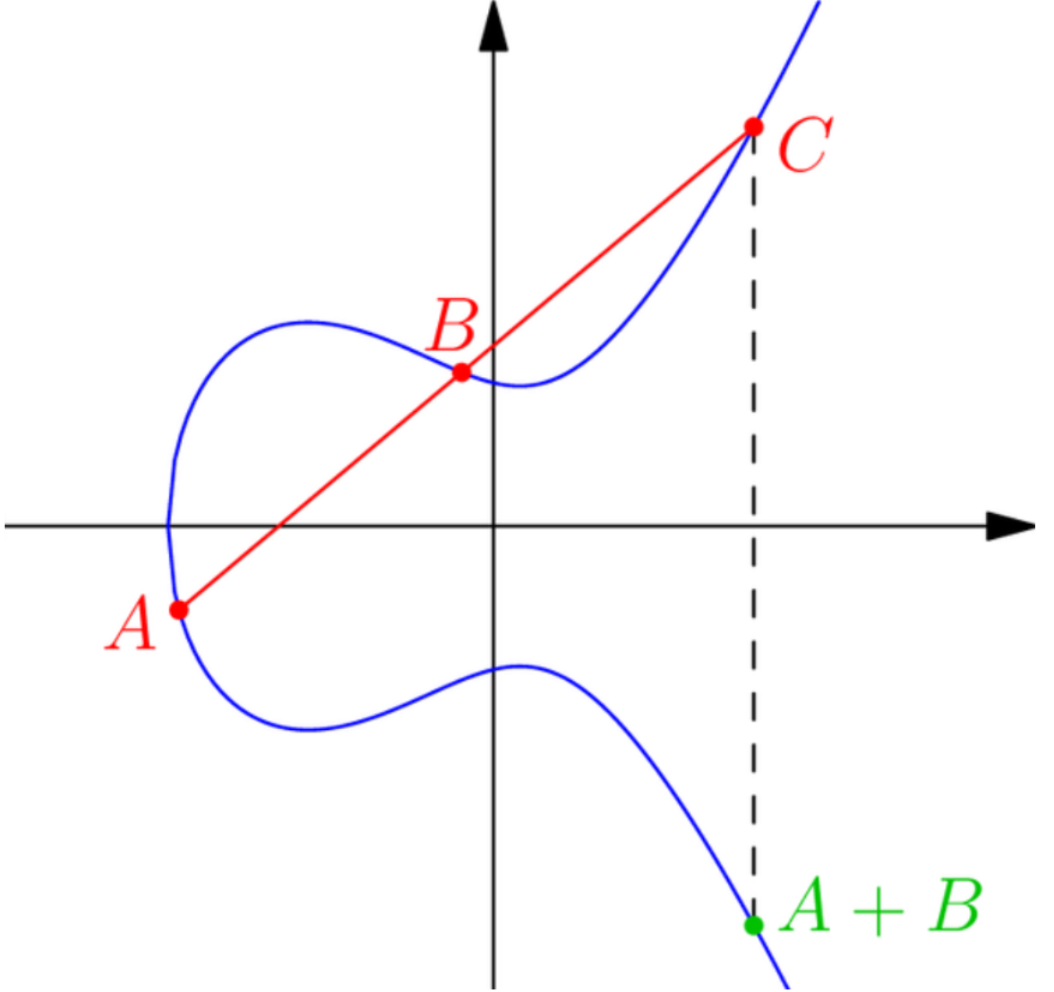
\includegraphics[width=\linewidth]{gfx/elliptic_curves_addition.png}
    \caption{Illustration of addition on elliptic curves}
    \label{fig:ell_curves_add}
\end{wrapfigure}

We define an addition operation for points on the elliptic curve.
The addition can be illustrated as shown in Figure \ref{fig:ell_curves_add}.
When two points $A$ and $B$ are added, first, the line that crosses both points will be found.
This line will cross the curve at another point, which is the point $-A+B$.
If we mirror the point on the x-axis, we get the point $A+B$ i.e the point resulting from the addition operation.

In case both points are the same, the line will be the tangent of the curve.
In case $A$ is added to $-A$, the line would be horizontal, thus not crossing the curve again.
The result of this operation is defined as the point at infinity $\mathcal{O}$.

When calculating with an elliptic curve, the concept is very similar to calculating in $mod$.
We have a generator Point $\mathcal{G}$ on $E$, which we will add to itself to produce new points in $E$.
The discrete logarithm problem on elliptic curves expresses \textit{how many times must $\mathcal{G}$ be added to itself to produce a Point Y?}:
$DLog_{\mathcal{G}}^{E}(Y)$ is the value $x$ for which $x\mathcal{G} = Y$.

If we had a given $Z_p^*$ and we could find an elliptic curve $E$ with the number of distinct elements $q$, such that $q$ is very close to $p$, this would be better than using a prime subgroup of $Z_p^*$.
The reason is that a prime subgroup of $Z_p^*$ would require us to choose $q << p$ because of the attacks shown in Section \ref{sec:index_caclulus} and \ref{sec:sec:number_field_sieve} work against subgroups of $Z_p^*$.
These smaller values are much faster to compute than bigger values.
The question now is whether given $Z_p^*$ it is actually possible to find an elliptic curve with its number of elements close to $p$.
Hasse's theorem shows that it is possible to find an elliptic curve with the number of elements relatively close to $p$ (with "only" up to $2\sqrt{p}$ distance to $p$):

$$
    p+1 - 2 \sqrt{p} \leq \; |E_{a,b}| \leq p+1 + 2 \sqrt{p}\;
$$

In practice, the value for $p$ and the elliptic curve is given.
Those are defined through standards published by e.g. the BSI.

The Youtube channel \url{https://www.youtube.com/@thenativeweb} also explains elliptic curves very nicely in the videos \textit{Architecture's Daily} episodes 91 to 95.

\section{Diffie-Hellman Key Exchange}\label{sec:diffie_hellman}

The Diffie-Hellman key exchange claims a way to generate a common secret key for two communication partners over a public channel.

\begin{figure}{h}
    \center
    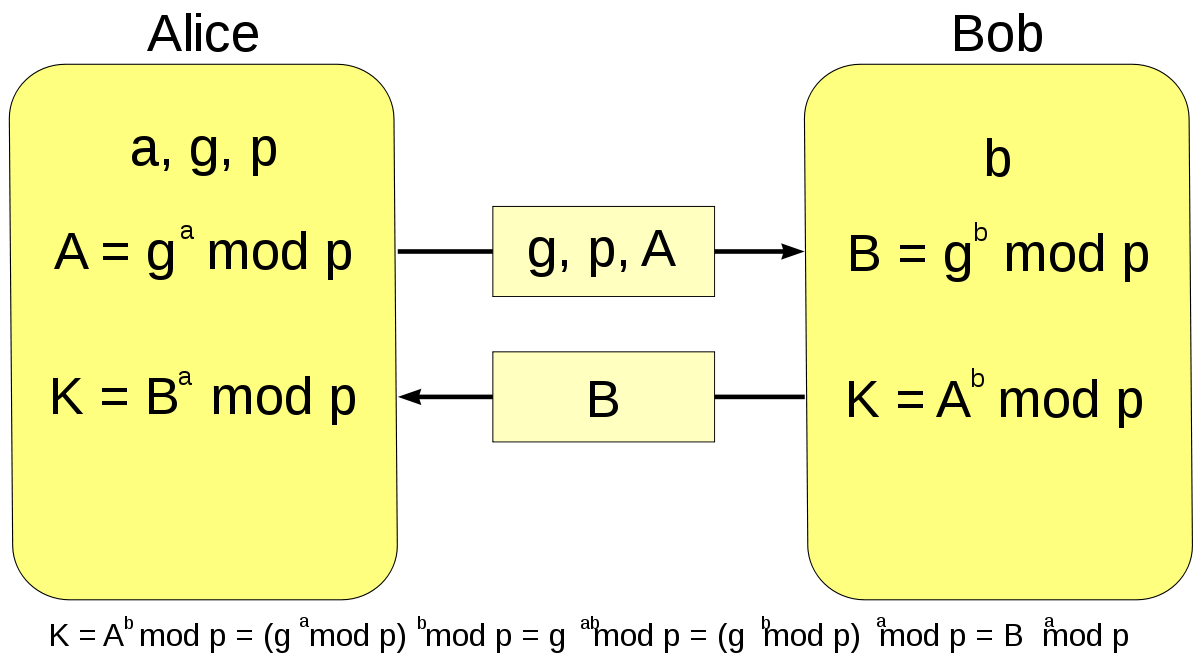
\includegraphics[width=\linewidth]{gfx/diffie-helman.png}
    \caption{Illustration of the Diffie-Hellman key exchange. Note that $g$ and $p$ can be generated by Alice, like shown here, or delivered by a third party (since both values are public).}
    \label{fig:diffie_hellman}
\end{figure}

\section{ElGamal Encryption}\label{sec:elgamal}

\begin{align*}
     & \underline{KGen(1^\lambda):}           &  & \underline{Enc(pk, (G,g,q), m):}   &  & \underline{Dec(sk, (Y,c)):} \\
     & (G,g,q) \leftarrow GroupGen(1^\lambda) &  & y \leftarrow\$ G                   &  & return c \cdot Y^{-sk}      \\
     & sk \leftarrow\$ G                      &  & \text{return } (g^y, pk^y \cdot m) &  &                             \\
     & pk \leftarrow g^{sk} \text{ in } G     &  &                                    &  &                             \\
     & \text{return } ((G,g,q), (sk, pk))     &  &                                    &  &
\end{align*}

ElGamal is IND-CPA if the DDH assumption (see section \ref{fig:DDH_assumption}) holds.
It is not IND-CCA because it has the following property:

$$
    Dec(sk, (Y, c \cdot r)) = Dec(sk, (Y, c)) \cdot r
$$

This holds because of $Dec(sk, (Y, c \cdot r)) = Y^{-sk} \cdot c \cdot r = g^{-sk \cdot y} \cdot g^{sk \cdot y} \cdot m \cdot r = m \cdot r = Dec(sk, (Y, c)) \cdot r$.
This allows an adversary to modify the ciphertext with a known outcome.
The adversary can then divide $r$ back out.
This way, ciphertexts $c$ can be decrypted without querying $c$ at the $DEC$ oracle, allowing us to compare them with an earlier from $ENC$ obtained $c$, this way breaking IND-CCA.

A further restriction of ElGamal is that all messages must be in the group $G$ and therefore have a certain length and structure.
Both problems are solved by ICIES.

\section{ICIES encryption}\label{sec:ICIES}

% TODO: differentiate between elgamal and DH

The ICIES (Elliptic Curve Integrated Encryption Scheme) encryption is a modern standardized version of the ElGamal encryption concept and uses Diffie-Hellman and the common key $K$ that it generates as the input for a PRF to create a key for symmetric encryption and authentication.

ICIES uses Diffie-Hellman for key exchange to generate two keys $(k_E, k_M)$, one for symmetric encryption and one for key exchange.
It then uses encrypt and MAC, which we have learned earlier.
Additionally, it uses a key derivation function (KDF).
The purpose of this function is simply to transform points on the elliptic curve into a binary representation that can be used as a key.
This means that KDF works like a hashing function.
For simplicity, in the following, we use the notation above $Z_p^*$ although ICIES in reality work with elliptic curves.
The operations of ICIES are formally defined as follows:

\begin{align*}
     & \underline{KeyGen(1^\lambda)}:         &  & \underline{Enc(pk, m)}                 &  & \underline{Dec(sk,(Y,c,\tau))}                              \\
     & (G,g,q) \leftarrow GroupGen(1^\lambda) &  & y             \leftarrow Z_p^*         &  & (k_E,k_M)                            \leftarrow KDF(Y^{sk}) \\
     & sk \leftarrow  G                       &  & Y             \leftarrow g^y           &  & \textit{if } MAC(k_M, c) \;!=\; \tau  \text{ return } \perp \\
     & pk  \leftarrow g^{sk}                  &  & (k_E, k_M)    \leftarrow KDF(pk^y)     &  & \text{return } SymDec(k_E,c)                                \\
     & \text{return } ((G,g,q), (pk,sk))      &  & c             \leftarrow SymEnc(k_E,m) &  &                                                             \\
     &                                        &  & \tau          \leftarrow MAC(k_M,c)    &  &                                                             \\
     &                                        &  & \text{return }(Y,c,\tau)               &  &                                                             \\
\end{align*}

$KeyGen$ is executed on the receiver side.
Then the public key must be published.
Afterwards, $Enc$ can be executed by senders.
The receiver can then decrypt the ciphertexts $(Y, c, \tau$) using $Dec$.

This is a so-called KEM-DEM hybrid encryption.
\textit{KEM-DEM} refers to a process of not explicitly encrypting the key, but already generating an encrypted key, which can be more performant than using a full asynchronous encryption to encrypt the symmetric key.
\textit{Hybrid} describes using an asymmetric system for generating a key and a faster symmetric system for encrypting payload data.


\section{Discrete Security Assumptions}

This chapter will explain the discrete security assumptions DL, CDH and DDH.
It can be proven that if DDH holds, CDH must hold and if CDH holds, DL must hold.
But we do not know the reverse.
All these assumptions are unbroken for more than 40 years know, however, not been proven either.

\subsection{DL (Discrete Logarithm) assumption}

\begin{wrapfigure}{r}{0.4\textwidth}
    \center
    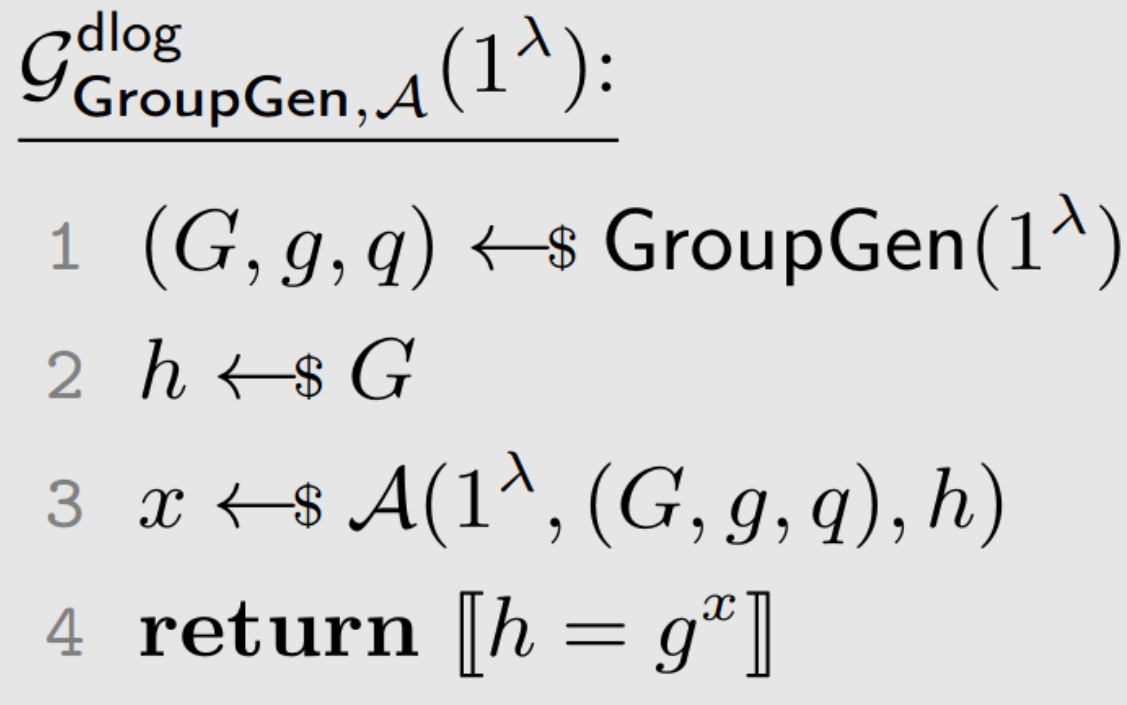
\includegraphics[width=\linewidth]{gfx/discrete_log_assumption.png}
    \caption{Game-based definition of the DL assumption.}
    \label{fig:DL_assumption}
\end{wrapfigure}

The discrete logarithm assumption is that given a group $(G,g,p)$ and a value $y \in G$, the discrete logarithm $DLog_g(y)$ is not efficiently computable.
This can be defined through the game shown in Figure \ref{fig:DDH_assumption}.
DL then states the following regarding the game for all $PPT$ adversarys $A$:

$$
    Pr[Exp_{GroupGen,A}^{dlog}(1^\lambda) = 1] \leq neg(\lambda)
$$


\subsection{CDH (Computational Diffie-Hellman) assumption}

\begin{wrapfigure}{r}{0.4\textwidth}
    \center
    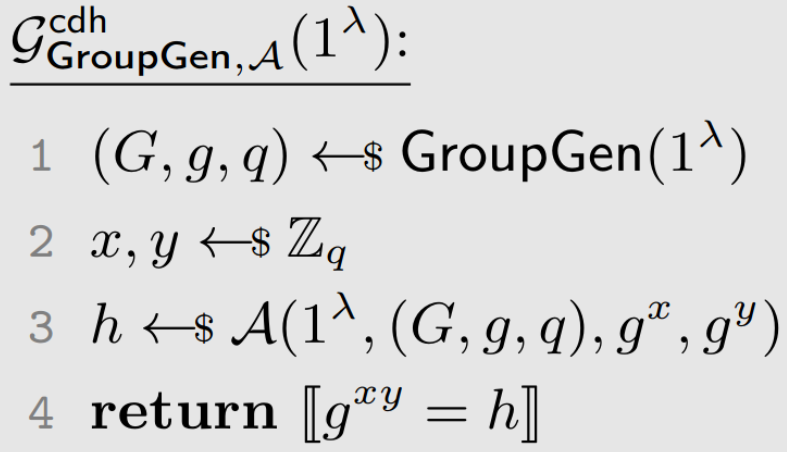
\includegraphics[width=\linewidth]{gfx/CDH_assumption.png}
    \caption{Game-based definition of the CDH assumption.}
    \label{fig:CDH_assumption}
\end{wrapfigure}


The computational Diffie-Hellman assumption states that given a group $(G,g,p)$ and two values $g^x$ and $g^y$, $g^{xy}$ cannot be computed efficiently (of course without knowing $x$ and $y$ but only knowing the powers).
If this holds, DL must also hold (can be shown by reduction).
This can be defined through the game shown in Figure \ref{fig:DDH_assumption}.
CDH then states the following regarding the game for all $PPT$ adversarys $A$:

$$
    Pr[Exp_{GroupGen,A}^{cdh}(1^\lambda) = 1] \leq neg(\lambda)
$$


\subsection{DDH (Decisional Diffie-Hellman) assumption}

\begin{wrapfigure}{r}{0.4\textwidth}
    \center
    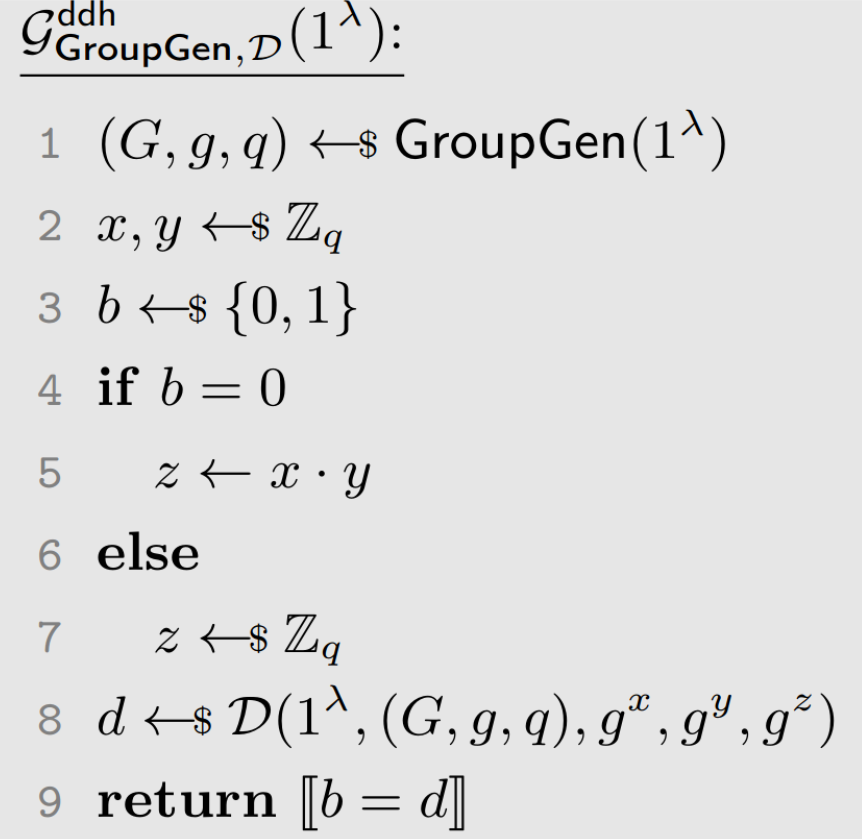
\includegraphics[width=\linewidth]{gfx/DDH_assumption.png}
    \caption{Game-based definition of the DDH assumption.}
    \label{fig:DDH_assumption}
\end{wrapfigure}

The decisional Diffie-Hellman assumption states that given $(G,p,g)$, $g^x$ and $g^y$, the two values $g^{xy}$ and $g^z$ can not be distinguished efficiently.
If this holds, CDH must also hold (can be shown by reduction).
This can be defined through the game shown in Figure \ref{fig:DDH_assumption}.
DDH then states the following regarding the game for all $PPT$ adversarys $A$:

$$
    Pr[Exp_{GroupGen,}^{ddh}(1^\lambda) = 1] \leq \frac{1}{2} + neg(\lambda)
$$

